%
% Chapter 2
%

\chapter{Theoretical Motivation}
\label{chap:theory}

The constituents of matter and their interactions at the most fundamental level is described by the Standard Model (SM) of particle physics. SM is a renormalizable quantum field theory with a $\suthree \times \sutwo \times \uone$ symmetry structure. SM incorporates electromagnetic, weak, and strong interactions. A brief theoretical overview of the elementary particles, the fundamental interactions, and the Higgs boson is presented in this chapter. The main shortcomings of the SM are listed at the end of the chapter.

\section{Phenomenological overview}

The intrinsic angular momentum (spin) of the elementary particles is used to classify them. Elementary particles with half-integer spin $(\frac{1}{2}, \frac{3}{2}, \frac{5}{2}, \ldots)$, are classified as fermions, while particles with integer spin (0, 1, 2, ...) are classified as bosons. Quarks and leptons constitute matter and are fermions. There are six quark flavors: up (u), down (d), strange (s), charm (c), bottom (b), and top (t). There are three different types of charged leptons: the electron (e), the muon (\Pgm), and the tau (\Pgt). Each lepton has its corresponding neutral partner: the electron neutrino ($\nu_{e}$), the muon neutrino ($\nu_{\Pgm}$), and the tau neutrino ($\nu_{\Pgt}$). The six flavors of leptons and quarks can be arranged into three generations.

Every fermion has a corresponding anti-particle with the same properties but opposite charges. Elementary particles of the SM can be seen in Figure \cite{fig:sm_particles}. All interactions, except gravitation, are part of the Standard Model and can be described as quantum fields. Their interactions are mediated by field quanta, the gauge bosons, which have spin 1. Quantum electrodynamics (QED) is the relativistic quantum field theory of electrodynamics. The weak interaction and electromagnetism can be unified to one theory, the electroweak theory. Quantum chromodynamics (QCD) is the theory of strong interaction.

\begin{figure}[htbp]
  \centering
  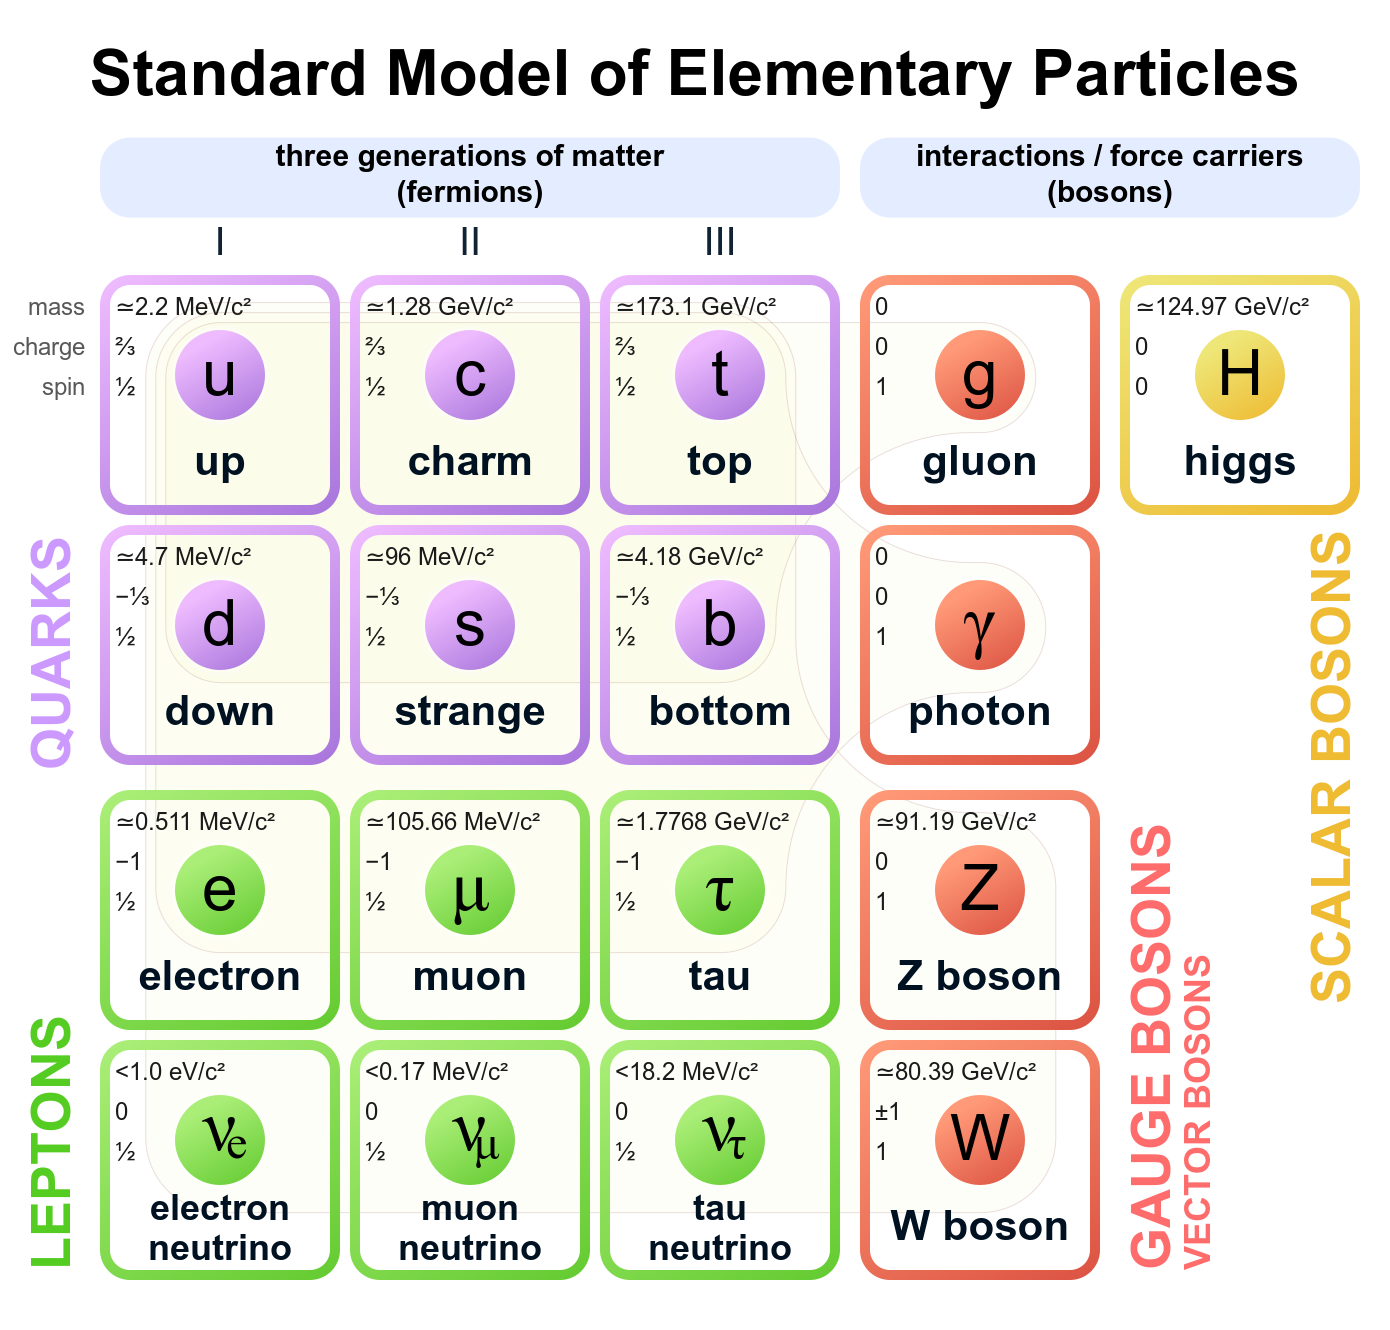
\includegraphics[width=0.8\textwidth]{plots/chapter2/sm_particles.png}
  \caption{Elementary particles of the Standard Model.}
  \label{fig:sm_particles}
\end{figure}

\subsection{Quantum electrodynamics}

Electromagnetism is described by Quantum electrodynamics (QED). QED interactions are mediated by the photon (\Pgg), which acts between electrically charged particles. The photon carries no electrical charge and is massless; therefore, electromagnetic interaction has an infinite range. Neutrinos are electrically neutral; thus, they do not interact via electromagnetic interaction. Up-type quarks have a charge of +2/3, while down-type quarks have a charge of -1/3. In QED, the elementary process is the emission and absorption of a photon: $\Pe^{-} \to \Pe^{-}+\Pgg$.

Initial and final-state particles define the physical process. The electromagnetic interaction processes can be described by combining two or more of the fundamental vertices to Feynman diagrams, representing mathematical expressions for calculating the probability amplitudes for a given process. Antiparticles are indicated as arrows going backward in time. Internal lines represent particles, which cannot be observed. The total probability amplitude of a process is proportional to all Feynman diagrams' squared sum, representing the same process. The calculated amplitudes can have infinite contributions. Renormalisation aims to separate the finite and infinite parts of the amplitude. Regularisation modifies the infinite observable by adding a parameter to make it finite. The resulting observable depends on the additional parameter, but it can be computed without divergences. The result is obtained by taking the parameter to its physical limit.

Virtual $\Pe^{+} \Pe^{-}$ pairs can spontaneously be produced around a ``bare'' electron reducing the observed charge at larger distances. This is referred to as charge screening. The fine-structure constant \aem characterizes the strength of the electromagnetic interaction between electrically charged particles. Each vertex introduces a factor proportional to $\sqrt{\aem}$, which depends on the energy scale. The value of \aem decreases with energy to a constant value of $\approx 1/137$ for long-distance interactions. Very precise QED predictions can be obtained using only lower-order diagrams, as the higher-order diagrams can be neglected due to the small value of \aem.

\subsection{Electroweak interaction}

The weak interaction is the mechanism of interaction between subatomic particles responsible for the radioactive decay of atoms. It is the only interaction that can change particles' flavor, and all fermions can interact weakly. Neutrinos can only interact via weak interaction. Three gauge bosons mediate the interaction: the $\PW^{+}$, $\PW^{-}$, and \PZ\, bosons. The \PZ\, boson can couple to two fermions of the same flavor, while the \PW\, boson couples to fermions of a different flavor. Also, both bosons can interact with each other. As the \PW\, bosons are electrically charged, they can additionally couple to photons. The weak interaction only acts over very short distances in the order of $10^{-18} \m$, because the \PZ\, and \PW\, bosons have large masses, about $91 \GeV$ and $80 \GeV$, respectively.

\subsection{Quantum chromodynamics}

Stong interaction is described by Quantum chromodynamics (QCD), which binds neutrons and protons into atomic nuclei. The strong interaction has a short-range in the order of $10^{-15} \m$. QCD interactions are mediated by a massless gauge boson called gluon (g), which acts on particles with a color charge. There are three such charges: red, green, and blue (r, g, b). Quarks are the only fermions which carry a color charge. A fundamental process of the strong interaction is the process, where a quark emits or absorbs a gluon: $\mathrm{q} \to \mathrm{q} + \mathrm{g}$. The gluons carry color themselves, a color, and an anti-color; therefore, they interact. There are eight types of gluons.

A bare quark is surrounded by a ``sea'' of virtual quarks and gluons. At shorter distances, corresponding to higher energies, the bare charge can be seen. This corresponds to the phenomenon of asymptotic freedom in which the interaction strength gets weaker with increasing energy and decreasing distance. The potential energy between two quarks is large enough to create a real quark-antiquark pair from the vacuum at a large distance. This process is known as fragmentation or hadronization. Two separating quarks always hadronize to colorless particles. The observation that only colorless bound states have been observed in nature is referred to as color confinement. The strong interaction binds quarks into composite states called hadrons. Hadrons can be classified into baryons, which are fermions, and mesons, which are bosons. Baryons are composed of three quarks. Mesons are composed of a quark and an anti-quark. The coupling strength of the strong interaction \as describes the dependence of the effective charge on the distance between them. In the lowest order, \as(Q) is given by:

\begin{equation}
  \alpha_{S}=\frac{6 \pi}{(33-2 n_{f}) \ln (Q / \Lambda_{\mathrm{QCD}})}
\end{equation}

where Q is the momentum transfer in a given process, $n_{f}$ the number of flavors which can participate in the process, and $\Lambda_{\mathrm{QCD}}$ corresponds to the energy boundary of hadronization. For $Q \approx \Lambda_{\mathrm{QCD}}$ quarks and gluons interact strongly and form hadrons, while \as(Q) becomes smaller for $Q \gg \Lambda_{\mathrm{QCD}}$ and quarks and gluons interact with each other only weakly. At low energies, perturbative methods cannot investigate the theory due to the large coupling strength.

\subsection{The Higgs boson}
In the SM, the gauge bosons must have no mass; however, \PW\, and \PZ\, bosons have non-zero mass. They receive their mass by interacting with the Higgs field and via the Higgs mechanism. Also, the fermions receive mass via this mechanism. The Higgs boson (H) is the field quanta of the Higgs field and has spin-0. The Higgs boson's fundamental vertices with the fermions, the gauge bosons (V) of the weak interaction, and its self-interactions can be seen in Figure \cite{fig:h_vertices}. It couples to two fermions of the same type, two \PW\, or \PZ\, bosons, and further Higgs bosons.

\begin{figure}[htbp]
  \centering
  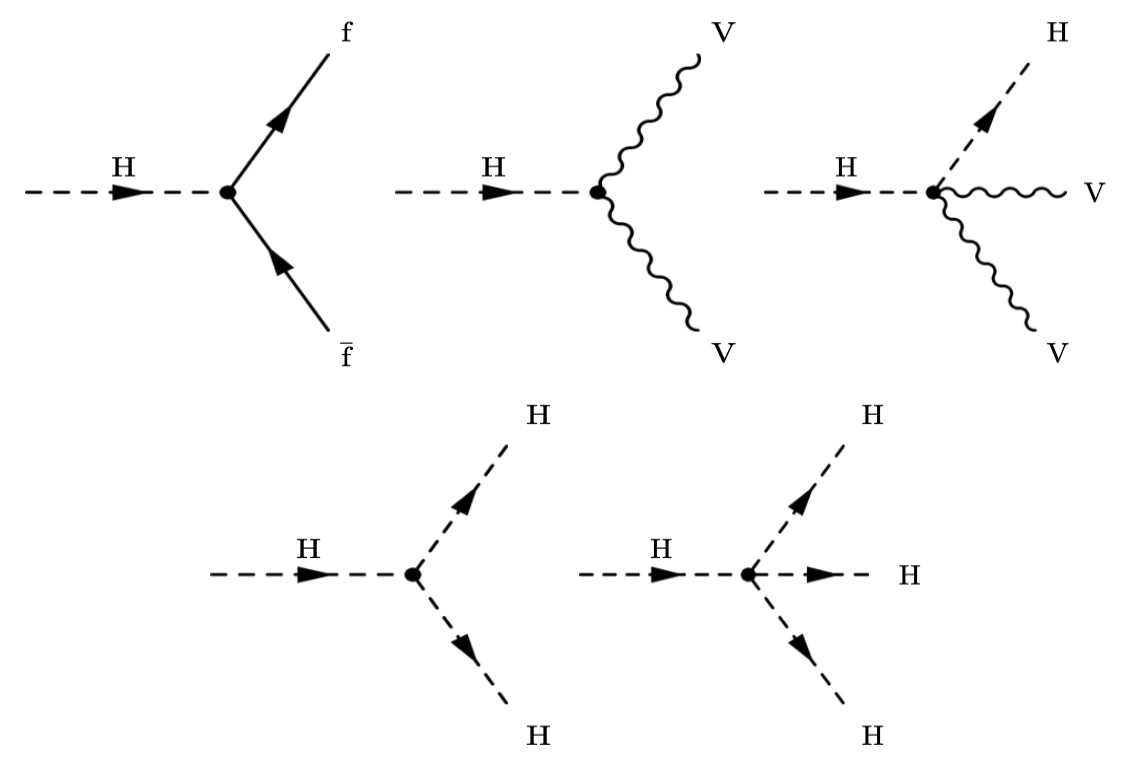
\includegraphics[width=0.8\textwidth]{plots/chapter2/h_vertices.png}
  \caption{Fundamental vertices of the Higgs boson. Fermions are denoted $\text{f}$, anti-fermions are denoted $\bar{\text{f}}$, and Gauge bosons of the weak interaction are denoted $\text{V}$.}
  \label{fig:h_vertices}
\end{figure}

\section{Overview of theoretical building blocks}
The Standard Model is a renormalizable quantum field theory. It has a $\suthree \times \sutwo \times \uone$ symmetry structure. Understanding the general, abstract details of structures is the aim of group theory. The corresponding Lagrangian of the theory describes the dynamics of a system. A type of quantum field theory is gauge theory, where gauge fields are introduced by requiring symmetry under local transformations. Finally, the idea of spontaneous symmetry breaking is discussed.

Group theory: A group $(\mathrm{G}, \star)$ is a set of objects G and some operations $\star$ on those objects. A set of elements $g_{i}$ is a group under some operation if the group axioms are satisfied: closure, associativity, the existence of an identity element, and an inverse element. A group is Abelian if the elements of the group commute under the group operation $(g_{i} \star g_{j}=g_{j} \star g_{i})$. Groups that are not Abelian are called non-Abelian.

The order n of the group is given by the number of elements in the group. A group can be represented by $n \times n$ matrices. A special type of groups are Lie groups, which are parameterized by one or more continuous variables. Transformations of elements $\in \mathbb{C}$ can be described as matrices R. These matrices are unitary if the Hermitian conjugate is also the inverse of the transformation, $R^{\dagger}=(R^{*})^{T}=R^{-1}$. A set of such $n \times n$ matrices forms the unitary group $\mathrm{U}(n)$, which preserves the norm under transformations, thus the probability amplitude. Some of these unitary matrices $R$ have a determinant $\operatorname{det}|R|=1$. The volume is preserved under such transformations. Such matrices form the special unitary group $\mathrm{SU}(n)$.

Lagrangian formalism: Its Lagrangian gives the information about the dynamics of a system as a function of generalized coordinates $q$ and their time derivatives $\dot{q}$. In classical physics, the Lagrangian is defined as the kinetic energy $T$ minus the potential energy $V$:

\begin{equation}
  L=T(q, \dot{q})-V(q)
\end{equation}

Fields are functions of spacetime. In field theory, the Lagrangian is replaced by the Lagrangian density $L$, which is a function of the fields $\phi(x^{\Pgm})$ in the system and their derivatives $\partial_{\mu} \phi$. The action $S$ of the system is defined as:

\begin{equation}
  S=\int \mathrm{d}^{4} x \mathcal{L}
\end{equation}

Quantum field theory: Quantum field theory (QFT) is a relativistic quantum theory of interactions. Particles are interpreted as fields, and other particles, the gauge bosons mediate forces between particles. In quantum mechanics, space is treated as an operator, while time is treated as in classical physics, as a parameter. However, space and time have to be treated in the same way for a relativistic theory. This is solved in QFT by quantizing in a new way. The fields are reinterpreted no longer as states but as operators parameterized by the spacetime coordinates. Commutation relations are imposed on the field operators. It is impossible to measure both the field and its time rate of change simultaneously to infinite precision at the same spacetime point. The state with the lowest possible energy level is called a vacuum. Acting on the vacuum with a field operator produces a state with some energy. The Lorentz transformations known from special relativity are elements of the Lorentz group. This group contains two copies of the SU(2) group, where the SU(2) group represents quantum mechanical spin. There are different representations, which are characterized by the value j, the spin of the particle. Consequently, a representation $(j, j^{\prime})$ of the Lorentz group is characterised by two values j and $j^{\prime}$ for each SU(2) subgroup. There are three physically acceptable irreducible representations of the Lorentz group:
\begin{itemize}
\item the $(0, 0 )$ scalar representation acting on scalars
\item the $(\frac{1}{2}, 0) \oplus(0, \frac{1}{2} )$ left-handed/right-handed spinor representations acting on spinors
\item the $(\frac{1}{2}, \frac{1}{2} )$ vector representation acting on vectors.
\end{itemize}

There are two types of spinors, left-handed $\Psi_{L}$ and right-handed $\Psi_{R}$, which transform the same under rotations, but they transform differently under boosts. Some fundamental properties of these objects are outlined in the following.

Scalar fields are spin-0 fields. Previously, spin was defined as intrinsic angular momentum. Spin is not a rotation in spacetime but the spinor space of SU(2). Complex scalar fields have the form $\phi=\phi_{1}+i \phi_{2}$, with two real degrees of freedom. The fields $\phi$ and $\phi^{\dagger}$ are treated independently. The Lagrangian density is given as a function of both the fields and their derivatives.

Spinor fields $\Psi$ are spin-1/2 fields and consist of four complex fields $\Psi_{i}$:

\begin{equation}
  \Psi=\left(\begin{array}{l}
  \Psi_{1} \\
  \Psi_{2} \\
  \Psi_{3} \\
  \Psi_{4}
  \end{array}\right), \Psi^{\dagger}=(\Psi_{1}^{*}, \Psi_{2}^{*}, \Psi_{3}^{*}, \Psi_{4}^{*})
\end{equation}

The adjoint spinor $\bar{\Psi}=\Psi^{\dagger} \gamma^{0}$ has to be defined to have Lorentz invariant terms in the Lagrangian density. The matrices satisfy the anti-commutation relation (Clifford algebra):

\begin{equation}
  \left\{\gamma^{\mu}, \gamma^{\nu}\right\}=\gamma^{\mu} \gamma^{\nu}+\gamma^{\nu} \gamma^{\mu}=-2 \eta^{\mu \nu} \mathbb{1}
\end{equation}

with Minkowski metric $\eta^{\mu \nu}$. The Lagrangian density is given as a function of the fields $\Psi, \bar{\Psi}$ and their derivatives. Parity transformations $\Lambda_{P}$ are one type of Lorentz transformations, which switch the handedness of a coordinate frame. Left-handed spinors are transformed into right-handed spinors under parity transformations. To be Lorentz invariant, spinor fields $\Psi$ should have a left-handed and a right-handed component, with the adjoint field of a left-handed spinor field $\bar{\Psi}_{L}$ being the same field as the right-handed spinor field $\Psi_{R}$:

\begin{equation}
  \bar{\Psi}_{L}=\Psi_{R}, \quad \bar{\Psi}_{R}=\Psi_{L}
\end{equation}

The projection operators $P_{\pm}$ are the projection operators onto the left- and right-handed parts of the field $\Psi$:

\begin{equation}
  P_{+} \Psi=\Psi_{R}, \quad P_{-} \Psi=\Psi_{L}
\end{equation}

Another important transformation is the charge conjugation: $\Psi \to C \bar{\Psi}^{T}=-i \gamma^2 \Psi^{*}$, which swaps the charge of the field. Vector fields \amu have spin 1. They have four components that transform as a spacetime vector under Lorentz transformations. Lorentz invariant terms are:

\begin{equation}
  \amu A^{\mu}, \quad (\partial_{\mu} A_{\nu})(\partial^{\mu} A^{\nu}), \quad (\partial_{\mu} A^{\mu})(\partial_{\nu} A^{\nu})
\end{equation}

The fundamental fermions are represented as spinor fields, while gauge bosons are represented as vector fields in QFT. Combining the Lagrangian densities of both fields leads to two fields, which do not interact with each other. An interaction term has to be added, which mixes both fields. Such a term can be introduced using gauge theory.

Gauge theory: A type of field theories are gauge theories, which are theories in which the Lagrangian is invariant under a continuous local transformations group. For example, a spinor field can be transformed with the global U(1) transformation $\Psi \to \mathrm{e}^{i \alpha} \Psi$, with being a real parameter. The transformation is just a phase and acts on the field in the same way at every point in spacetime. A local transformation has a spacetime dependence. In this example of the U(1) transformation, would depend on spacetime: $\alpha=\alpha(x^{\mu})$. The same type's possible transformations are associated with a Lie group, the theory's symmetry group. All elements of a group can be expressed in terms of the group generators.

First, a Lagrangian density is defined for a fermion field with an equation of motion that satisfies the Dirac equation. This Lagrangian density is not invariant under a local gauge transformation. A new vector field \amu has to be introduced, called gauge field, for each group generator $T_{a}$ to ensure invariance under the local group transformations, called gauge invariance. The vector field can be expressed with the group generators, $\amu=\amu^{a} T_{a}$, and the gauge bosons are the quanta of these fields. The derivative operator $\partial_{\mu}$ in the Lagrangian density is replaced by the covariant derivative $D_{\mu}$, which is $\partial_{\mu}$ with a term proportional to a gauge field.

Local transformations can be written in form of $U=\mathrm{e}^{i g \chi_{a}(x^{\mu}) T_{a}}$, where g is a real parameter, the coupling constant, and $\chi_{a}(x^{\mu})$ is a scalar with a spacetime dependence. The covariant derivative is then given by $D_{\mu}=\mathbb{1}^{n \times n} \partial_{\mu}+i g \amu^{a} T_{a}$. Interaction terms are introduced by the second term of the covariant derivative. A kinetic term, proportional to the fields' derivatives, can be introduced for including dynamics of the vector field. Vector fields with mass break the local gauge symmetry; therefore, the vector fields are massless, i.e., have no terms proportional to $\amu A^{\mu}$.

All fundamental interactions of the SM can be derived from this general principle of local gauge invariance. As the SM \PW\, and \PZ\, bosons are massive, a mechanism is needed to acquire mass. This mechanism is the Higgs mechanism and combines the principles of gauge theory and spontaneous symmetry breaking.

Spontaneous symmetry breaking: Gauge fields can acquire mass in case of broken local symmetry. Breaking a global symmetry always results in massless bosons, called Goldstone bosons \cite{Goldstone:1961eq, Goldstone:1962es}. Consider a complex scalar field with a Lagrangian which has a local \uone symmetry and a potential $V(\phi^{\dagger}, \phi)$ with the vacuum $V_{minimum}$ given by the circle $|\phi|=v$. Choosing a single ground state breaks the system's symmetry and is considered ``spontaneous'' because there are no external means by which this occurs. The theory can be rewritten in terms of the new vacuum, by a change of basis. The field is expanded around the constant vacuum value, writing the fields in terms of fluctuations around the chosen vacuum.

The Higgs mechanism combines the principles of gauge invariance with spontaneous symmetry breaking. For a local U(1) symmetry, the vacuum can be chosen so that the vacuum is real and that $\phi$ is always real; therefore, $\phi$ can be expanded as $\phi=v+h$, with h being a real scalar field. Breaking the local \uone symmetry results in a real scalar h with a mass, and the field \amu, originating from the local gauge symmetry, acquires mass. The Higgs mechanism introduces mass into a theory by breaking the local symmetry. A scalar Higgs field h is introduced, and the gauge field of the broken symmetry acquires mass. In general, gauge fields corresponding to group generators of broken symmetries acquire mass, while those corresponding to generators of unbroken symmetries do not acquire a mass.

\section{The Standard Model}
The Standard Model is a non-Abelian gauge theory based on the group $\col \times \iso \times \hyp$, where $C$ stands for color, $Y$ stands for the hypercharge to distinguish \hyp from the \uone of QED, and $L$ indicates that the interaction only involves left-handed states. QCD is based on the group \col, which corresponds to rotations in color space. Eight gauge bosons, called gluons, mediate the strong interaction. Fermions are described as a triplet of spinors which differ in color

\begin{equation}
  \psi=\left(\begin{array}{l}
  \psi_{r} \\
  \psi_{b} \\
  \psi_{g}
  \end{array}\right)
\end{equation}

\begin{equation}
  \begin{array}{|l|l|c|c|}
    \hline \text { Group } & \text { Operation } & \text { Coupling } & \text { Vector field } \\
    \hline \hyp & \text { phase rotation } & g^{\prime} & \bmu \\
    \hline \iso & \text { rotation in the weak isospin } & g & W_{\mu}^{a} \\
    \hline \col & \text { rotation in the colour } & g_{S} & G_{\mu}^{a} \\
    \hline
  \end{array}
\end{equation}

There are eight gauge fields $G_{\mu}^{a}$ with the gluons being the field quanta, which mediate the strong interaction. Leptons do not interact under the SU(3) color group, but quarks do. The electroweak theory is based on the group $\iso \times \hyp$. Only left-handed fields interact under \iso; therefore, only a left-handed neutrino is needed. Left-handed and right-handed fields can interact under the \hyp group, therefore charged leptons have to exist in a left-handed and a right-handed state. Left-handed \iso doublets

\begin{equation}
  \psi_{L}=\left(\begin{array}{l}
  \nu_{e} \\
  e_{L}
  \end{array}\right)
\end{equation}

and right-handed \iso singlets $e_{R}$ are introduced. There are three gauge fields $W_{\mu}^{a}$ for \iso, and one gauge field \bmu for \hyp. Table 2.1 gives an overview of the symmetry groups in the SM. The gauge fields are all massless, but the gauge bosons of the weak theory have mass. Masses can be generated for the \PW\, and \PZ\, bosons via the Higgs mechanism by breaking the electroweak symmetry. Also, quarks and leptons acquire mass via the Higgs mechanism by applying the mechanism to the corresponding fields.

A Higgs field is introduced, which is a complex scalar $\iso \times \hyp$ doublet field. Breaking the vacuum's symmetry via the Higgs mechanism results in a broken theory with two separate forces: the broken weak theory and the unbroken theory of electromagnetism associated with the $\uone_{em}$ symmetry of QED. The new fields $\amu, W_{\mu}^{\pm}$, and $Z_{\mu}^{0}$ are linear combinations of the vector fields of $\iso \times \hyp$:

\begin{equation}
  \begin{aligned}
    \amu=\sin \theta_{W} W_{\mu}^{3}+\cos \theta_{W} \bmu \\
    W_{\mu}^{\pm}=(W_{\mu}^{1} \mp i W_{\mu}^2) / \sqrt{2} \\
    Z_{\mu}^{0}=-\cos \theta_{W} W_{\mu}^{3}+\sin \theta_{W} \bmu
  \end{aligned}
\end{equation}

with the weak mixing angle or Weinberg angle $\theta_{W}=\tan ^{-1}(\frac{g^{\prime}}{g}), \sin \theta_{W}=g^{\prime} / \sqrt{g^2+g^{\prime 2}}$ and $\cos \theta_{W}=g / \sqrt{g^2+g^{\prime 2}}$ in terms of the couplings $g$ of \iso and  $g^{\prime}$ of \hyp. The weak mixing angle relates the strength of the weak and electromagnetic interaction, which are mediated by the massive \PW\, and \PZ\, bosons, and the massless photon which is the field quanta of \amu. Furthermore, the electroweak coupling $e$ of $\uone_{em}$ is given by $e \equiv g \sin \theta_{W}$.

\section{Electroweak symmetry breaking and the Higgs boson}
In the SM, the weak gauge bosons acquire mass via the Higgs mechanism. An arbitrary scalar potential

\begin{equation}
  V(\Phi)=\mu^2 \Phi^{\dagger} \Phi+\lambda(\Phi^{\dagger} \Phi)^2
\end{equation}

with a self-interacting \sutwo scalar complex field $\Phi$ is introduced, where \Pgm is the mass term of the field. The complex Higgs doublet $\Phi$ has four degrees of freedom, and it is composed of CP-even and CP-odd components $\phi^{0}$ and $a^{0}$, and the complex charged component $\phi^{+}$:

\begin{equation}
  \Phi=\frac{1}{\sqrt{2}}\left(
  \begin{array}{c}
    \sqrt{2} \phi^{+} \\
    \phi^{0}+i a^{0}
  \end{array}\right)
\end{equation}

For $\mu^2<0$, the scalar doublet's neutral component acquires a non-zero vacuum expectation value (VEV) $v$. Then $\phi^{0}$ can be expanded as $\phi^{0}=v+H$ with:

\begin{equation}
  \Phi=\frac{1}{\sqrt{2}}\left(
  \begin{array}{c}
    0 \\
    v + H
  \end{array}\right)
\end{equation}

The $\col \times \iso \times \hyp$ is broken into a $\col \times \uone_{em}$ symmetry. After symmetry breaking, there are three massless Goldstone bosons, which can be identified with three degrees of freedom of the Higgs field. The Higgs field couples to the \PW\, and B fields through the covariant derivative in the kinematic term. As a result, the Goldstone bosons mix with the gauge bosons of the corresponding generators of broken symmetries, and the physics \PW\, and \PZ\, gauge bosons acquire masses:

\begin{equation}
  M_{\mathrm{W}}^2=\frac{g^2 v^2}{4}, \quad M_{\mathrm{Z}}^2=\frac{(g^{\prime 2}+g^2) v^2}{4}
\end{equation}

There is one remaining degree of freedom, which is the Higgs boson. The mass of this new scalar (spin-0) particle is given by $m_{H}=\sqrt{2 \lambda} v$, with the self-coupling parameter. The sign of $\mu^2=-\lambda v^2$ is crucial for the electroweak symmetry. The expectation value of the Higgs field is fixed by the precise measured Fermi coupling GF: $v=(\sqrt{2} G_{F})^{-1 / 2} \approx 246 \mathrm{GeV}$. The SM also acquire fermion masses through the new interactions between the Higgs field and the fermion, the Yukawa interactions. The charge conjugated Higgs doublet $\tilde{\Phi}$ is needed to allow interactions with up-type quarks. Then, the Lagrangian of the Yukawa term is given by:

\begin{equation}
  \mathcal{L}_{\text {Yukawa }}=-\hat{\lambda}_{d_{i j}} \bar{q}_{L_{i}} \Phi d_{R_{j}}-\hat{\lambda}_{u_{i j} \bar{q}_{L_{i}}} \tilde{\Phi} d_{R_{j}}-\hat{\lambda}_{\ell_{i j}} \bar{\ell}_{L_{i}} \Phi e_{R_{j}}+\text {h.c.}
\end{equation}

where $h.c.$ indicates the Hermitian conjugated terms and $\hat{\lambda}$ are $3 \times 3$ matrices for the up and down-type quarks, and the charged leptons. Under electroweak symmetry breaking,

the Higgs field acquires a VEV and the fermion mass eigenstate basis is chosen, so that the Higgs interactions are diagonalised: $\hat{\lambda}_{f_{i j}} \to \lambda_{f_{i}} \delta_{i j}$. The fermions acquire a mass, which is given by $m_{f_{i}}=\lambda_{f_{i}} v / \sqrt{2}$, with the corresponding Yukawa coupling $\lambda_{f}$. Furthermore, they couple to the Higgs boson

\begin{equation}
  \mathcal{L}_{\text {Yukawa }}=-g_{H_{f f}} \bar{\Psi} \Psi H
\end{equation}

with $g_{H_{f f}}=\frac{m_{f}}{v}$. As the masses of the fermions are known, the only free parameter is the SM's Higgs boson mass. The Higgs boson is the most recently discovered fundamental particle. It was discovered by the ATLAS and CMS collaborations in 2012 \cite{Chatrchyan:2013lba}. Its mass and full width were measured to be $M_{\mathrm{H}}=125.09 \pm 0.24 \mathrm{GeV}$ and $\Gamma<1.7 \mathrm{GeV}$.

\section{Main shortcomings of the Standard Model}
The Standard Model is a very successful theory, and the electroweak theory has been verified over a wide range of energies. It was crowned with the discovery of the Higgs boson by the ATLAS and CMS collaborations in 2012. However, the SM is an incomplete theory as it does not incorporate gravitation. In SM's original formulation, neutrinos are strictly massless because there is no Dirac mass term due to the absence of right-handed neutrinos. There is no Majorana mass term due to the conservation of baryon and lepton number. However, neutrino experiments have established the existence of neutrino oscillations, transitions between the different neutrino flavors. This is evidence for neutrino mixing and nonzero neutrino masses. Astrophysical observations imply an unknown type of matter and energy, called dark matter and dark energy, which cannot be explained within the SM. Space observatories like Planck have studied the fluctuations in the spectrum of the relic cosmic microwave background (CMB) and have established the existence of cold dark matter \cite{Ade:2015xua}. Also, the CP-violating effects of the SM cannot explain the large difference between matter and anti-matter in the universe. Furthermore, the flavor structure is not explained in the theoretical description of the SM. There is a large number of free parameters, such as masses and mixing parameters. The Higgs mechanism can explain how masses are introduced in the SM, but it cannot explain its values.

\section{Lepton flavor violating decays of the Higgs boson}
The Standard Model is considered to be an effective theory up to a certain scale $\Lambda$. One shortcoming is that the flavor structure is not incorporated in the theoretical description of the SM.
There are three main puzzles in the SM related to flavor \cite{Raidal:2008jk}:
\begin{itemize}
\item The replication of the generation constitutes.
\item There is no principle underlying the formation of the Yukawa matrices describing the SM Yukawa interactions.
\item The peculiar pattern of fermion masses and mixing cannot be explained.
\end{itemize}
New physics could explain some of the symmetries and open questions. Grand Unification Theories (GUTs) try to unify all known interactions but gravity in a single gauge group, while extra dimensions could link flavor to this extra dimension's geometry. A simple extension of the Higgs sector with at least two Higgs doublets could add additional CP-violation. A Higgs boson was discovered in 2012, whose properties are compatible with the SM Higgs boson, within experimental uncertainties. Its mass has been measured by the ATLAS and CMS collaborations and found to be $125.09 \pm 0.24 \mathrm{GeV}$. After the discovery of the Higgs boson, its nature has to be investigated by measuring its properties, including its couplings to charged leptons. Charged leptons acquire mass through Yukawa interactions with the Higgs field, as described in Chapter 2. In the SM, the Yukawa interaction matrix can be diagonalized in the mass basis. Thus, LFV decays of the Higgs boson are forbidden. Extensions of the SM, such as multi-Higgs doublet models, can introduce LFV Yukawa couplings. Multi-Higgs doublet models have in general tree-level Higgs-mediated flavor changing neutral currents leading to LFV Yukawa couplings. LFV Yukawa couplings can also be introduced in composite Higgs models \cite{Blankenburg:2012ex} and models with extra dimensions.

In the following, a short review on LFV decays of the Higgs bosons is given, which was the status at the time when the search was started. It is described how new physics can introduce LFV Yukawa-couplings and how low-energy measurements constrain them. Finally, it is described how LFV decays of the Higgs boson can be measured at the LHC and which sensitivity is expected, including observed upper limits on the branching fraction \cite{Khachatryan:2015kon}.

\subsection{Introduction of lepton flavor violating decays}
The Higgs mechanism is responsible for the masses of the gauge bosons and the fermions. First, it is discussed how charged leptons gain mass in the SM. Yukawa interactions mediate interactions between charged leptons with the Higgs field; therefore, the corresponding Yukawa matrix structure in the mass basis is afterward discussed. Then, it is explained how LFV Yukawa couplings can be introduced considering an effective field theory approach. Finally, an overview is given on the structure of the Yukawa matrix for charged leptons in general. Decay widths and branching fractions of the LFV decay in terms of the corresponding Yukawa couplings are also shown.

Yukawa couplings of charged leptons in the SM Charged leptons acquire a mass via the Higgs mechanism, introduced in Section 2.4. A direct mass term is not gauge invariant, but interactions of the charged leptons $\ell$ to the scalar Higgs field $\phi$ can be introduced with the following term:

\begin{equation}
  \mathcal{L}_{\mathrm{SM}}=-\lambda_{i j} L_{L}^{i} \Phi \ell_{R}^{j}+\text {h.c.}
\end{equation}

where with $\bar{L}_{L}^{i}=(\bar{\nu}_{\ell}^{i}, \bar{\ell}_{L}^{i})$, are the \iso doublets, and $\bar{\ell}_{R}^{i}$ the weak singlets with the indices $i, j$ running over generations. After electroweak symmetry breaking, the Higgs doublet can be written in terms of the vacuum expectation value $v$ and the physical Higgs boson H:

\begin{equation}
  \Phi=\frac{1}{\sqrt{2}}\left(\begin{array}{c}0 \\ v+H \end{array}\right)
\end{equation}

leading to the following Lagrangian:

\begin{equation}
  \begin{aligned}
    \mathcal{L}_{\mathrm{SM}} &=-\frac{\lambda_{i j}}{\sqrt{2}}(v+H) \overline{\ell_{L}}^2 \ell_{R}^{j}+h.c. \\
    &=-\frac{\lambda_{i j}}{\sqrt{2}} v[\overline{\ell_{L}^{i} \ell_{R}^{j}}-\frac{\lambda_{i j}}{\sqrt{2}}[\overline{\ell_{L}^{i} \ell_{R}^{j} H}]+h.c.
  \end{aligned}
\end{equation}

where the term proportional to $\bar{\ell}_{L}^{i} \ell_{R}^{j}$ is the mass term of the charged leptons and the term proportional to $\bar{\ell}_{L}^{i} \ell_{R}^{j}H$ describes the Yukawa interactions. The mass matrix m, with $m_{ij}=\frac{\lambda_{ij}}{\sqrt{2}} v$, can be diagonalised using the matrices $V_{L}$ and $V_{R}$:

\begin{equation}
  m=\left(\begin{array}{ccc}
  m_{e} & 0 & 0 \\
  0 & m_{\Pgm} & 0 \\
  0 & 0 & m_{\Pgt}
  \end{array}\right)=\frac{1}{\sqrt{2}} V_{L} \lambda V_{R}^{\dagger} v=\frac{\lambda^{m}}{\sqrt{2}} v
\end{equation}

where $\lambda^{m}=V_{L} \lambda V_{R}^{\dagger}$ is written in terms of the mass basis. The Yukawa interaction matrix $\text{Y}$ can also be written in terms of the mass basis:

\begin{equation}
  \mathrm{Y}=V_{L} \frac{\lambda}{\sqrt{2}} V_{R}^{\dagger}=\frac{\lambda^{m}}{\sqrt{2}}=\frac{m}{v}=\left(\begin{array}{ccc}
  \Yee & 0 & 0 \\
  0 & \Ymm & 0 \\
  0 & 0 & \Ytt
  \end{array}\right)
\end{equation}

which is also diagonal. Thus, there are no LFV Yukawa interactions in the SM.

Dimension-6 operators: If the Higgs field is the only field that causes electroweak symmetry breaking and if the particle spectrum is consisting only out of SM particles, including the Higgs boson, up to some energy scale $\Lambda \gg 200 \mathrm{GeV}$, additional heavy fields can be integrated out, leading to an effective field theory. Terms including higher-dimension operators, can be added to the SM Lagrangian, which has dimension four. An effective Lagrangian can be written including dimension-6 operators

\begin{equation}
  \mathcal{L}_{eff}=\mathcal{L}_{SM}+\sum_{nij} \frac{\alpha_{n}^{ij}}{\Lambda^2} O_{n}^{i j}
\end{equation}

where $i, j$ denote flavor indices, n runs over the number of independent operators, $\Lambda$ is the scale of new physics, and $\alpha_{n}^{i j}$ are coefficients \cite{DiazCruz:1999xe}. This effective Lagrangian describes the effects of new physics at the electroweak scale in a model-independent way. A dimension-5 operator can generate neutrino masses. However, this operator does not generate LFV interactions for the Higgs boson. The dimension-6 operator $O_{L \phi}^{i j}=(\Phi^{\dagger} \Phi)(\bar{L}_{i} \ell_{R j} \Phi)$ is a Yukawa-type operator that only generates LFV interactions of the Higgs boson. It also contributes to the fermion mass matrices. These contributions have to be included in the fermion mass matrices. Then, the mass matrices are diagonalized. Finally, the interaction term of the Lagrangian is written in terms of the mass basis. Including the Yukawa-type operator to the Lagrangian leads to the following additional term:

\begin{equation}
  \Delta \mathcal{L}=-\frac{\lambda_{i j}^{\prime}}{\Lambda^2}(\Phi^{\dagger} \Phi)(\bar{L}_{L}^{i} \ell_{R}^{j} \Phi)+h . c .
\end{equation}

where $\lambda_{i j}^{\prime}$ is the coefficient $\alpha_{n}^{i j}$ of the dimension-6 operator $O_{L \phi}^{i j}$.

Electroweak symmetry breaking leads to the following Lagrangian terms:

\begin{equation}
  \begin{aligned}
    \Delta \mathcal{L} &=-\frac{\lambda_{i j}^{\prime}}{\Lambda^2}(\frac{v+H}{\sqrt{2}})^2 \bar{\ell}_{L}^{i} \ell_{R}^{j}(\frac{v+H}{\sqrt{2}}) \\
    &=-\frac{\lambda_{i j}^{\prime}}{\Lambda^2} \frac{1}{(\sqrt{2})^{3}}(v^{3}+3 v^2 H+3 v H^2+H^{3}) \bar{\ell}_{L}^{i} \ell_{R}^{j} \\
    &=-\frac{1}{\sqrt{2}} \frac{\lambda_{i j}^{\prime}}{2 \Lambda^2}(v^{3} \overline{\ell_{L}^{i} \ell_{R}^{j}}+3 v^2 \overline{\ell_{L}^{i} \ell_{R}^{j} H}+3 v \bar{\ell}_{L}^{i} \ell_{R}^{j} H^2+\bar{\ell}_{L}^{i} \ell_{R}^{j} H^{3})
  \end{aligned}
\end{equation}

where term proportional to $\overline{\ell_{L}^{i}} \ell_{R}^{j}$ leads to an additional mass term of the charged leptons and the term proportional to $\overline{\ell_{L}^{i}} \ell_{R}^{j}H$ adds a further Yukawa-interaction term. Thus, the mass term of the effective Lagrangian $\mathcal{L}_{\text {mass }}$ is the sum of the SM mass term and the additional contribution:

\begin{equation}
  \begin{aligned}
    \mathcal{L}_{\text {mass }} &=\mathcal{L}_{\text {mass}, \mathrm{SM}}+\Delta \mathcal{L}_{\text {mass }} \\
    &=-(\frac{\lambda_{i j}}{\sqrt{2}} v+\frac{1}{\sqrt{2}} \frac{\lambda_{i j}^{\prime}}{2 \Lambda^2} v^{3}) \bar{\ell}_{L}^{i} \ell_{R}^{j} \\
    &=-\frac{1}{\sqrt{2}}(\lambda_{i j}+\frac{v^2}{2 \Lambda^2} \lambda_{i j}^{\prime}) v \bar{\ell}_{L}^{i} \ell_{R}^{j}
  \end{aligned}
\end{equation}

The term of the effective Lagrangian which describes the Yukawa interactions, $\mathcal{L}_{\text {Y}}$, is given by:

\begin{equation}
  \begin{aligned}
    \mathcal{L}_{Y} &=\mathcal{L}_{Y, \mathrm{SM}}+\Delta \mathcal{L}_{Y} \\
    &=-(\frac{\lambda_{i j}}{\sqrt{2}}+\frac{1}{\sqrt{2}} \frac{\lambda_{i j}^{\prime}}{2 \Lambda^2} 3 v^2) \bar{\ell}_{L}^{i} \ell_{R}^{j} H \\
    &=-\frac{1}{\sqrt{2}}(\lambda_{i j}+3 \frac{v^2}{2 \Lambda^2} \lambda_{i j}^{\prime}) \bar{\ell}_{L}^{i} \ell_{R}^{j} H
  \end{aligned}
\end{equation}

The mass matrix of the charged leptons can be diagonalized as for the SM using other matrices $V_{L}, V_{R}$:

\begin{equation}
  \sqrt{2} m=V_{L}[\lambda+\frac{v^2}{2 \Lambda^2} \lambda^{\prime}] V_{R}^{\dagger} v
\end{equation}

Then, the Yukawa interaction matrix can be written in terms of the mass basis:

\begin{equation}
  \begin{aligned}
    \sqrt{2} \mathrm{Y} &=V_{L}[\lambda+3 \frac{v^2}{2 \Lambda^2} \lambda^{\prime}] V_{R}^{\dagger} \\
    &=\frac{\sqrt{2} m}{v}+V_{L} 2 \frac{v^2}{2 \Lambda^2} \lambda^{\prime} V_{R}^{\dagger} \\
    &=\frac{\sqrt{2} m}{v}+\frac{v^2}{\Lambda^2} V_{L} \lambda^{\prime} V_{R}^{\dagger} \\
    &=\frac{\sqrt{2} m}{v}+\frac{v^2}{\Lambda^2} \hat{\lambda}
  \end{aligned}
\end{equation}

where $m$ is the diagonal mass matrix and $\hat{\lambda}=V_{L} \lambda^{\prime} V_{R}^{\dagger}$. The first term is the Yukawa term of the SM, while the second term can introduce non-diagonal terms as $\hat{\lambda}$ is in principle an arbitrary non-diagonal matrix, leading to Yukawa couplings \Yij given by:

\begin{equation}
  \mathrm{Y}_{i j}=\frac{m_{i}}{v} \delta_{i j}+\frac{v^2}{\sqrt{2} \Lambda^2} \hat{\lambda}_{i j}
\end{equation}

with possible LFV Yukawa interactions.

LFV Yukawa couplings: The inclusion of LFV Yukawa interactions was discussed by introducing a dimension-6 operator to the Lagrangian. There are several possible additional terms to the Lagrangian due to new physics, which prevent the diagonalization of the mass matrix and the Yukawa matrix at the same time. Another example is theories with more than one Higgs doublet, where the scalar fields can mix, leading to a neutral Higgs boson within general LFV Yukawa interactions. Thus, the Yukawa term of the Lagrangian for the charged leptons in the mass basis is after the electroweak symmetry breaking in general given by:

\begin{equation}
  \mathcal{L}_{\text {Yukawa }}=-m_{i} \bar{\ell}_{L}^{i} f_{R}^{i}-Y_{i j} \bar{\ell}_{L}^{i} \ell_{R}^{j} \mathrm{H}+\text { h.c. }
\end{equation}

where \Yij are the entries of the Yukawa matrix:

\begin{equation}
  \mathrm{Y}=\left(\begin{array}{ccc}
  \Yee & \Yem & \Yet \\
  \Yme & \Ymm & \Ymt \\
  \Yte & \Ytm & \Ytt
  \end{array}\right)
\end{equation}

which can have LFV Yukawa couplings \Yij. LFV Yukawa couplings allow LFV decays of the Higgs boson. The decay width of LFV Higgs boson decays is

\begin{equation}
  \Gamma(\mathrm{H} \to \ell_{i} \ell_{j})=\frac{m_{\mathrm{H}}}{8 \pi}(|\mathrm{Y}_{j i}|^2+|\mathrm{Y}_{i j}|^2)
\end{equation}

Using the decay width of the LFV decay, the branching fraction of the LFV Higgs boson decay can be derived when contributions of the other LFV decays are negligible

\begin{equation}
  \mathrm{B}(\mathrm{H} \to \ell_{i} \ell_{j})=\frac{\Gamma(\mathrm{H} \to \ell_{i} \ell_{j})}{\Gamma(\mathrm{H} \to \ell_{i} \ell_{j})+\Gamma_{\mathrm{SM}}}
\end{equation}

where \gsm is the total width of the Higgs boson in the SM. Non-negligible contributions to the total decay width from other LFV Higgs boson decays would have to be added to \gsm for estimating the branching fractions.

In the SM, the Higgs boson couples to all particles according to their mass. In the presence of new physics, LFV Yukawa couplings might be related closely to the fermion mass matrices, reflecting the observed fermion mass hierarchy \cite{Cheng:1987rs}. Then, the LFV couplings have a hierarchical structure given by $\Delta_{i j} \sqrt{\mathrm{m}_{i} \mathrm{m}_{j}}$, where $i, j$ are the generation indices, and $\Delta_{i j}$ is related to the mass mixing. Mass corrections to the lepton masses coming from mass mixing are assumed to be small in the so-called natural assumption. SM Yukawa couplings are taken for the flavor diagonal couplings. Thus, LFV branching fractions can be expressed in terms of SM ones:

\begin{equation}
  \mathrm{B}_{\text {nat}}(\mathrm{H} \to i j)=\mathrm{B}_{\mathrm{SM}}(\mathrm{H} \to i i) \cdot \frac{\mathrm{m}_{j}}{\mathrm{m}_{i}}
\end{equation}

with $\Gamma_{\mathrm{tot}} \approx \Gamma_{\mathrm{SM}}$, \BHij being the natural branching fraction and \BHsm being the branching fraction for the SM Higgs boson decay to two leptons $i$. The LFV branching fractions are expected to be of the same size or smaller than \BHij. Larger total widths lead to a smaller branching fraction. A naturalness assumption referred to as theoretical naturalness limit can also be derived for the Yukawa couplings \Yij:

\begin{equation}
  |\Yji \Yij| \lesssim \frac{\mathrm{m}_{i} \mathrm{m}_{j}}{\mathrm{v}^2}
\end{equation}

with $v$ being the vacuum expectation value of the Higgs boson.

\subsection{Constraints from low-energy measurements}

Constraints on LFV decays of the Higgs boson have been derived using low-energy measurements and certain assumptions on the value of flavor diagonal Yukawa couplings. In the following, constraints from several low-energy measurements on LFV Yukawa-couplings are discussed. Diagrams that can contribute to the low-energy measurements are shown. The results of the measurements and assumptions used to derive constraints on the LFV Yukawa-couplings are given. Finally, an overview of all constraints is given.

Constraints from LFV decays \liljg: LFV Yukawa couplings also contribute to LFV decays of type \liljg, where $i, j$ are flavor indices with $i \neq j$. One-loop diagrams and two-loop diagrams of this process are shown in Figure \cite{fig:tmg}. Constraints on the LFV Yukawa couplings of the Higgs boson with $m_{H} = 125$ GeV can be derived assuming SM values for \Ytt, \Ymm, and $\mathrm{Y}_{\mathrm{tt}}$.

\begin{figure}[htbp]
  \centering
  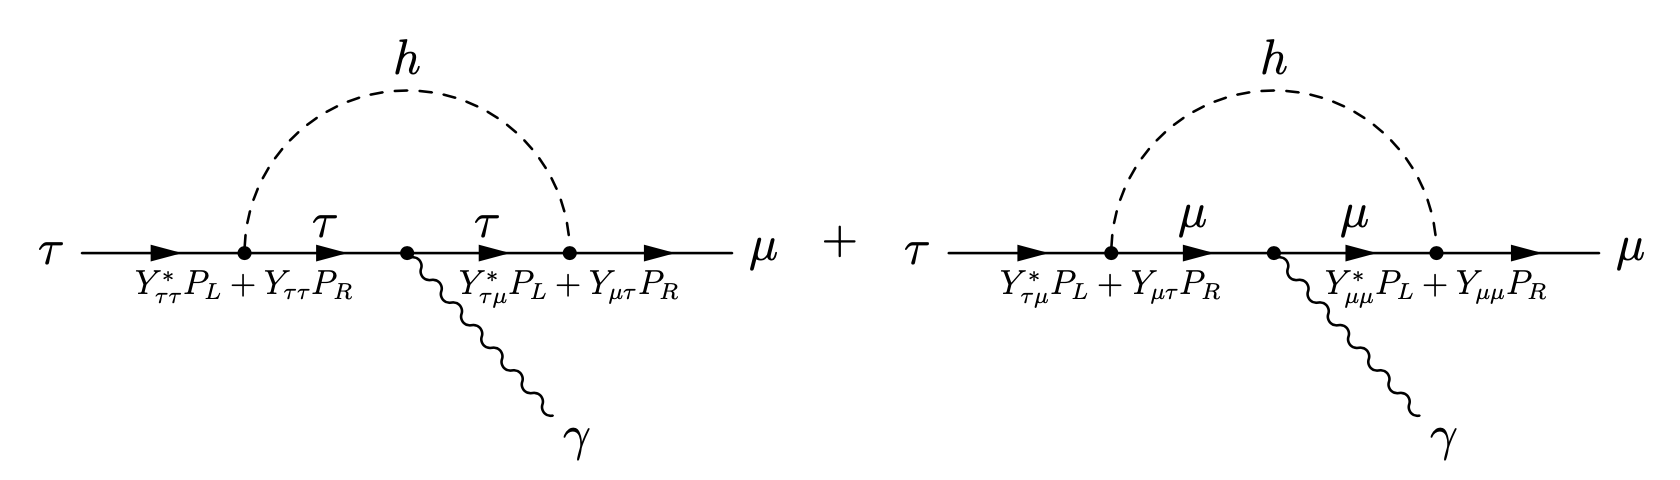
\includegraphics[width=0.8\textwidth]{plots/chapter2/1loop.png} \\
  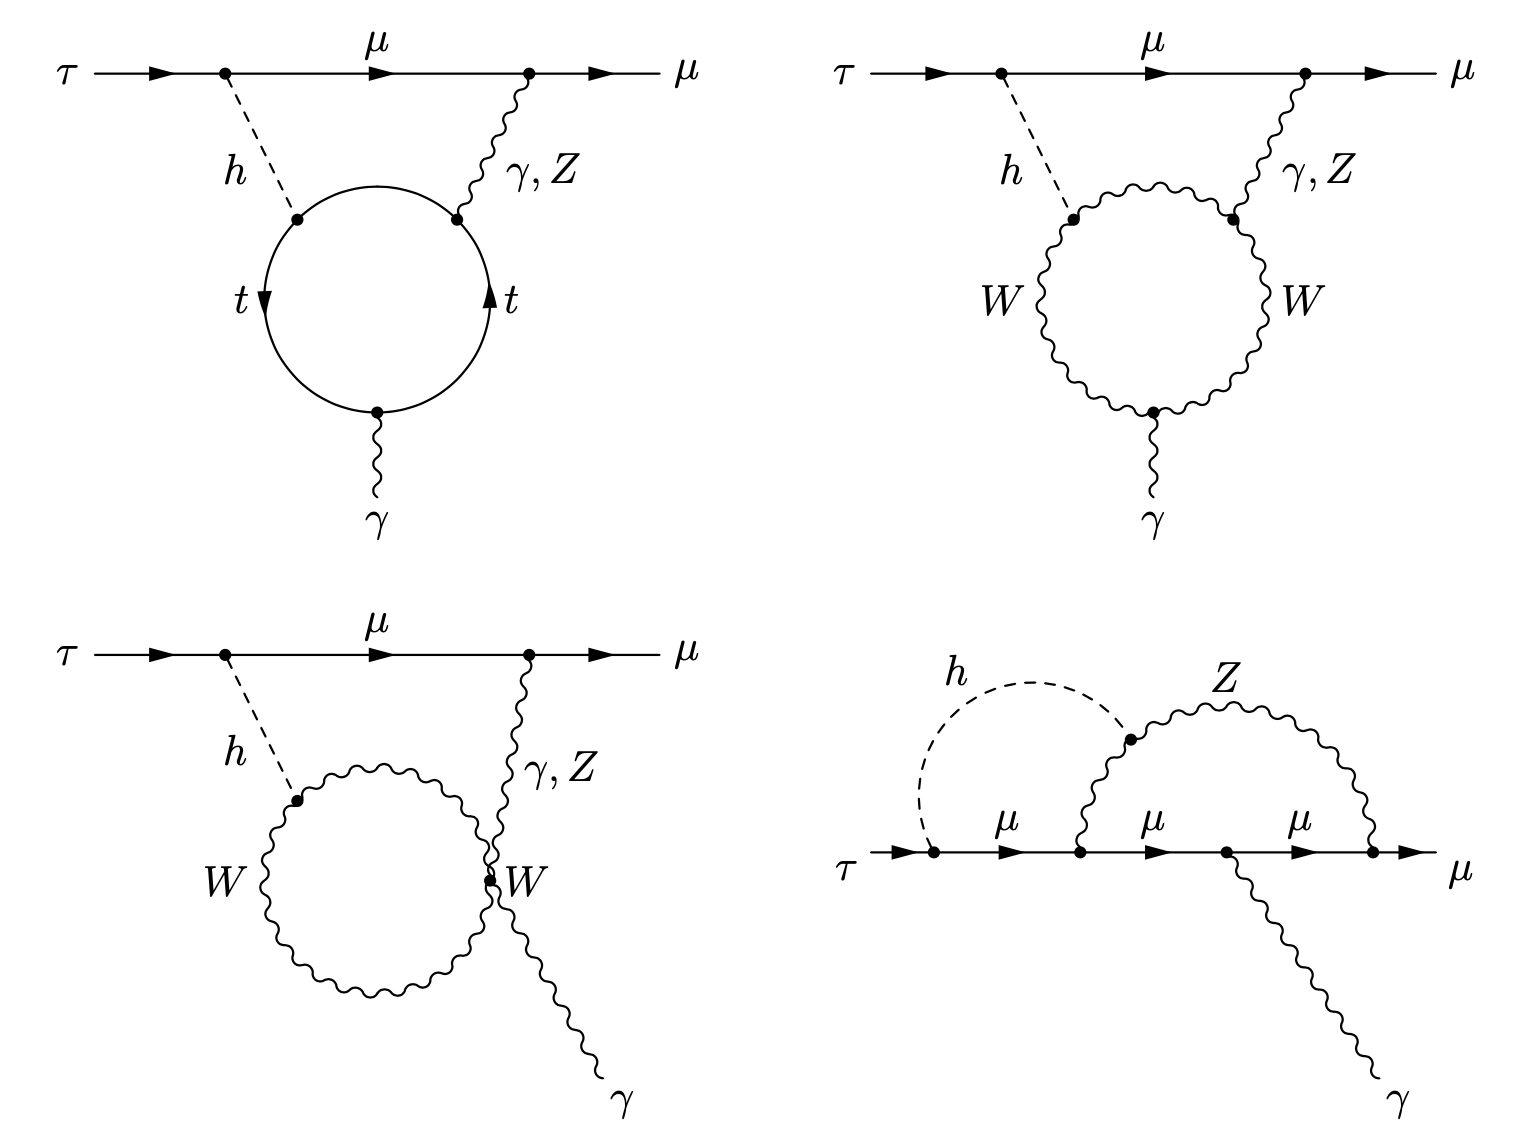
\includegraphics[width=0.8\textwidth]{plots/chapter2/2loop.png}
  \caption{Diagrams contributing to the flavor violating decay $\Pgt \to \Pgm \Pgg$, mediated by a Higgs boson with flavor violating Yukawa couplings.}
  \label{fig:tmg}
\end{figure}


Experimental upper bounds on the branching fractions $\mathrm{B}(\liljg )$ used for deriving constraints are summarised in Table \cite{tab:indirect}. Constraints of type $\sqrt{|\Yij|^2+|\Yji|^2}$ can be derived. A further constraint on $(|\Ytm \Yet|^2 + |\Ymt \Yte|^2)^{1 / 4}$ can be obtained from $\Pgm \to \Pe \Pgg$ by setting \Yme and \Yem to zero.

\begin{equation}
  \begin{array}{|l|c|c|c|}
    \hline \text { Decay } & \mathrm{B}(\Pgt \to \Pgm \Pgg) & \mathrm{B}(\Pgt \to \Pe \Pgg) & \mathrm{B}(\Pgm \to \Pe \Pgg) \\
    \hline \text { Experimental bound } & <4.4 \times 10^{-8} & <3.3 \times 10^{-8} & <2.4 \times 10^{-12} \\
    \hline
  \end{array}
\end{equation}

Constraints from LFV decays \ltl: LFV decays of type \ltl can constrain the LFV Yukawa couplings. Such decays have been searched for, and the experimental upper bounds on the branching fractions are summarised in Table 3.2. The previous assumptions on the mass of the Higgs boson and flavor diagonal Yukawa couplings were used to derive constraints on the LFV Yukawa couplings. \PZ\, boson contribution to the LFV decay $\Pgt \to \Pgm$, described in are neglected, as it turns out that their contributions are negligible \cite{Goto:2015iha}.

Constraints from muonium-antimuonium oscillations: The bound state $\Pgm^{+} \Pe^{-}$ is called muonium (M) and can oscillate to the $ \Pe^{+} \Pgm^{-}$ bound state called antimuonium ($\bar{M}$). An upper constraint on the conversion probability $P(M \to \bar{M})<8.3 \times 10^{-11}$ \cite{Willmann:1998gd} was derived by the muonium-antimuonium conversion spectrometer (MACS) experiment at PSI. The time-integrated conversion probability depends on the mass splitting between the two mass eigenstates of the mixed $M-\bar{M}$ system, which depends on $|Y_{\Pgm e}+Y_{e \Pgm}^{*}|$ \cite{Harnik:2012pb}.

A correction factor $S_{B} = 0.35$, accounting for the splitting of the muonium states in the magnetic field of the detector, was applied on the conversion probability $P(M \to \bar{M})<8.3 \times 10^{-11} / S_{B}$ when deriving the constraints on the LFV Yukawa couplings, leading to a weaker upper bound on the conversion probability. The correction factor depends on the conversion operator, and the smallest value was used to derive the constraints.

Constraints from magnetic and electric dipole moments: The muon's experimental value $g_{\Pgm}-2$ is more than three standard deviations above the SM prediction. Neglecting terms suppressed by $m_{\Pgm} / m_{\Pgt}$ or $m_{\Pgt} / m_{H}$, the LFV contribution to $g_{\Pgm}-2$ due to the one-loop diagram has the form

\begin{equation}
  a_{\Pgm} \equiv \frac{g_{\Pgm}-2}{2} \propto \operatorname{Re}(\Ymt \Ytm)
\end{equation}

with the discrepancy between measurement and SM prediction having the size

\begin{equation}
  \Delta a_{\Pgm} \equiv a_{\Pgm}^{\mathrm{exp}}-a_{\Pgm}^{\mathrm{SM}}=(2.87 \pm 0.63 \pm 0.49) \times 10^{-9}
\end{equation}

where $a_{\Pgm}^{\mathrm{exp}}$ and $a_{\Pgm}^{\mathrm{SM}}$ are the measured and predicted value, respectively. The one-loop diagram can contribute to an electric dipole moment (EDM) of the muon if the LFV Yukawa couplings are complex. If the terms suppressed by $m_{\Pgm} / m_{\Pgt}$ or $m_{\Pgt} / m_{H}$ are neglected, the dependence on the LFV Yukawa couplings of the electric dipole moment $d_{\Pgm}$ is

\begin{equation}
  d_{\Pgm} \propto-\operatorname{Im}(\Ymt \Ytm)
\end{equation}

Constraints from \mte conversion in nuclei LFV Yukawa couplings can contribute to \mte conversion in nuclei via tree-level exchange of a Higgs boson and one-loop diagrams with a Higgs boson and a photon exchange. Two-loop contributions are larger than the one-loop ones, as they are only suppressed by the weak gauge coupling or \Ytt. Thus, they were taken into account for deriving the constraints on the LFV Yukawa couplings assuming SM values for the flavor diagonal Yukawa couplings, as described before. These Yukawa couplings have not been observed at the LHC up to today. Using these assumptions, the LFV decays of type \liljg give the strongest constraints.

Constraints on the LFV Yukawa couplings from low-energy measurements are summarised in Table \ref{tab:indirect} and Figure \ref{fig:yuk}. They were, in most cases, derived using certain assumptions regarding the flavor diagonal Yukawa couplings. These measurements constrain the branching fractions of LFV Higgs boson decays to \mutau or \etau to be $\lesssim \mathcal{O}(10^{-1})$, while the constraint for the decay to \emm is stronger and $\lesssim \mathcal{O}(10^{-8})$. Constraints on the branching fractions were derived under the assumption that only one of them contributes to the Higgs boson's total width, additionally to the SM total width.

\begin{table}[!hbpt]
  \centering
  \caption{Constraints on LFV Yukawa couplings from low-energy measurements \cite{Harnik:2012pb}.}
  \begin{tabular}{ccc}
    \hline
    \hline
    Channel                   & Coupling                   & Bound                 \\
    \hline
    $\Pgm \to \Pe \Pgg$       & $\sqrt{|\Yme|^2+|\Yem|^2}$ & $<3.6 \times 10^{-6}$ \\
    $\Pgm \to 3 \Pe$          & $\sqrt{|\Yme|^2+|\Yem|^2}$ & $\lesssim 3.1 \times 10^{-5}$ \\
    electron $g-2$            & Re(\Yem \Yme)              & $-0.019 \ldots 0.026$ \\
    electron EDM              & |Im(\Yem \Yme)|            & $<9.8 \times 10^{-8}$ \\
    $\Pgm \to$ \Pe conversion & $\sqrt{|\Yme|^2+|\Yem|^2}$ & $<1.2 \times 10^{-5}$ \\
    $M-\bar{M}$ oscillations  & $|\Yme+\Yem^{*}|$          & $<0.079$ \\
    \hline
    $\Pgt \to \Pe \Pgg$       & $\sqrt{|\Yte|^2+|\Yet|^2}$ & $<0.014$ \\
    $\Pgt \to 3 \Pe$          & $\sqrt{|\Yte|^2+|\Yet|^2}$ & $\leq 0.12$ \\
    electron $g-2$            & Re(\Yet \Yte)              & $-2.1 \ldots 2.9 \times 10^{-3}$ \\
    electron EDM              & |Im(\Yet \Yte)|            & $<1.1 \times 10^{-8}$ \\
    \hline
    $\Pgt \to \Pgm \Pgg$      & $\sqrt{|\Ytm|^2+|\Ymt|^2}$ & $<0.016$ \\
    $\Pgt \to 3 \Pgm$         & $\sqrt{|\Ytm|^2+|\Ymt|^2}$ & $\lesssim 0.25$ \\
    muon $g-2$                & Re(\Ymt \Ytm)              & $(2.7 \pm 0.75) \times 10^{-3}$ \\
    muon EDM                  & |Im(\Ymt \Ytm)|            & $-0.8 \ldots 1.0$ \\
    \hline
    $\Pgm \to \Pe \Pgg$       & $(|\Ytm \Yet|^2+|\Ymt \Yte|^2)^{1/4}$ & $<3.4 \times 10^{-4}$ \\
    \hline
    \hline
  \end{tabular}
  \label{tab:indirect}
\end{table}

\begin{figure}[htbp]
  \centering
  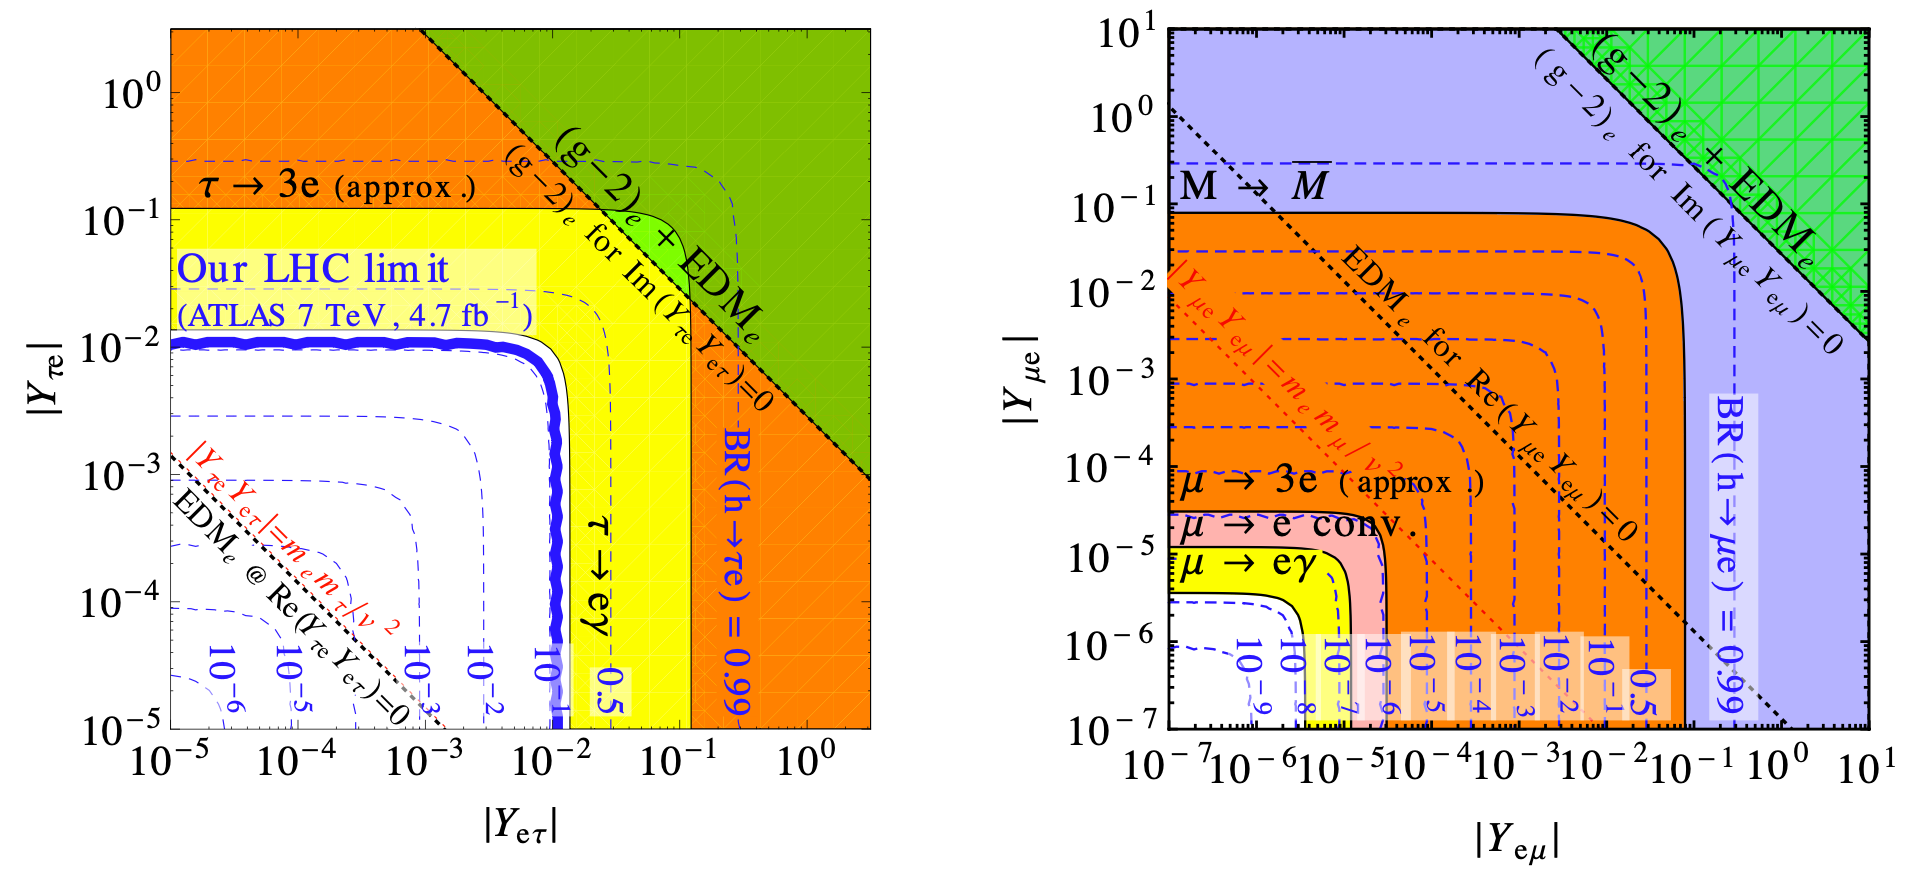
\includegraphics[width=0.8\textwidth]{plots/chapter2/Ymt.png} \\
  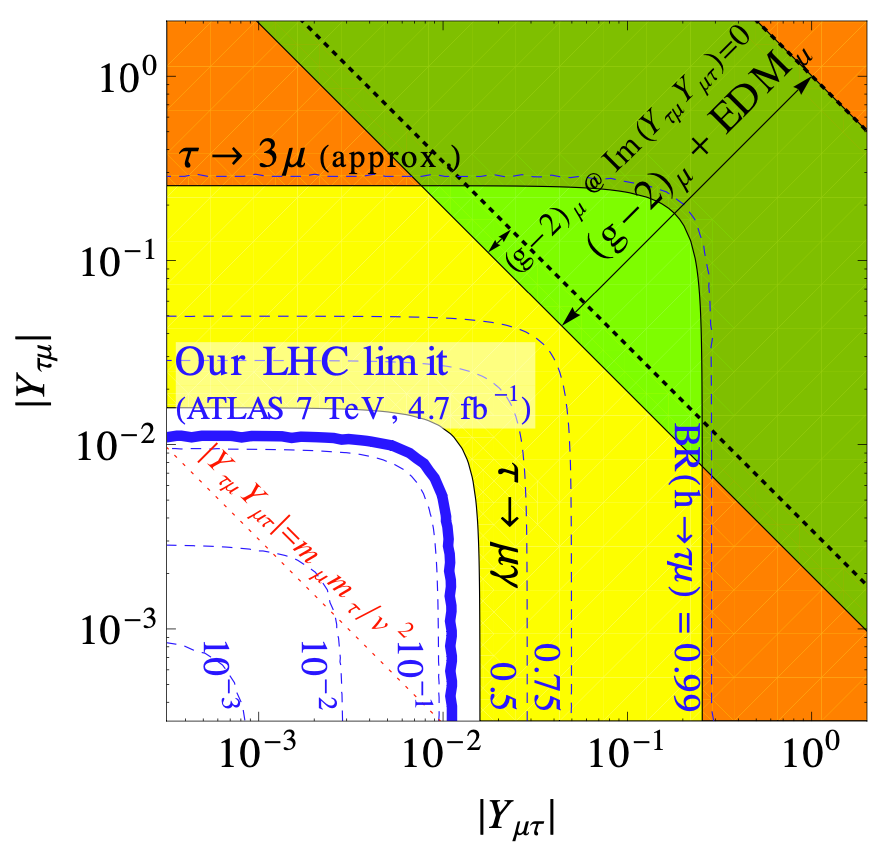
\includegraphics[width=0.4\textwidth]{plots/chapter2/Yem.png}
  \caption{Constraints on the LFV Yukawa couplings for a 125 GeV Higgs boson. The diagonal Yukawa couplings are approximated by their SM values. Shaded regions show the constraints from low-energy measurements. The thin red dotted lines show the theoretical naturalness limits $|\Yji \Yij| \lesssim \frac{\mathrm{m}_{i} \mathrm{m}_{j}}{\mathrm{v}^2}$.}
  \label{fig:yuk}
\end{figure}

\subsection{Lepton flavor violating decays of the Higgs boson at the LHC}
A Higgs boson was discovered in 2012, whose properties are compatible with the SM Higgs boson, within experimental uncertainties. Its mass has been measured by the ATLAS and CMS collaborations and found to be $125.09 \pm 0.24 \mathrm{GeV}$. The nature of the discovered Higgs boson has to be investigated by measuring its properties, including its couplings to charged leptons. In the following, SM production-mechanisms of the Higgs boson are discussed, relevant at the LHC. Possible LFV decays of the Higgs boson are presented. The size of the branching fractions on SM Higgs boson decays and the natural LFV branching fractions, Section 3.1, is discussed. Status is given about the upper limits on these decays' branching fraction, which was in July 2014.

Higgs boson production mechanisms: Gluon fusion (GF) and vector-boson fusion (VBF) are the dominant Higgs boson production-mechanisms \cite{deFlorian:2016spz}. Other production mechanisms have a lower cross-section; therefore, they can be neglected for this search.

LFV Yukawa couplings: LFV Yukawa couplings can introduce decays of the Higgs boson to \mutau, \etau, or \emm. Decays of the Higgs boson to \mutau or \etau can be split into a leptonic channel (\taue / \taum) and a hadronic channel (\tauh). The branching fractions of tau to a muon or an electron are $\sim 20 \%$, while $\sim 65 \%$ of the taus decay hadronically.

Taus have a short life-time of $\Pgt=(290.3 \pm 0.5) \times 10^{-15} \mathrm{s}$ and a decay length of $c \Pgt=87.03 \mu \mathrm{m}$ leading to a secondary vertex, which can be resolved within the CMS pixel tracking-detector. Muons, electrons, and hadronic taus can be reconstructed with the CMS detector. Neutrinos from tau decays lead to missing transverse energy \met. Feynman diagrams for \Hmue (a), \Hemu (c), and \Hem (e) lead to a signature with an isolated electron and an isolated muon of opposite charge in the CMS detector.

The last decay mode can be distinguished from the other Higgs boson decays by the absence of \ET due to neutrinos. Decays to \mue or \emu can be distinguished by the small angle between the lepton's direction from the tau decay and the direction of the missing transverse momentum $\sim \ET$, due to the neutrinos, for high momenta of the tau. Feynman diagrams for \Hmuhad (b), or \Hehad (d) have signatures with a hadronic tau and an isolated electron or muon, respectively. Their signature includes \ET as well due to the neutrino of the tau decay.

Tau decays to a lepton with the same flavor as the lepton of the Higgs boson decay. The channels \ee and \mm, are not considered because their signatures are very similar to Z-boson decays, leading to an overwhelming background of di-leptons for such processes.

Branching fractions: In the SM, the Higgs boson should couples to all particles according to their mass. The branching fraction for Higgs boson decays to taus is in the order of 6\%, and the branching fraction of the Higgs boson to muons is in the order of 0.02\%.

The LFV branching fractions are expected to be of the same size or smaller than \BHij using the natural assumption. Furthermore, LFV branching fractions \BHij can be expressed in terms of SM ones. Then, the LFV Higgs boson decay to \mutau should have a natural branching fraction in the order of 0.5\%, which is between decays to taus muons. LFV decays of the Higgs boson to \etau would have a smaller natural branching fraction in the order of $0.001\% = 10^{-5}$. Decays of the Higgs boson to \emm would even have a smaller natural branching fraction of the order $10^{-6}$.

Upper limits on LFV branching fractions: Low-energy measurements, described in Section 3.2, indirectly constrain branching fractions of the LFV Higgs boson decays to \mutau or \etau to be smaller than 10\%, which is larger than their natural branching fractions. The constraint for decays to \emm is in the order of $10^{-8} \m$, which is smaller than the natural branching fraction. These constraints were derived, assuming flavor changing neutral currents to be dominated by Higgs boson contributions; therefore, LFV effects could be canceled by other new physics effects leading to weaker limits. Direct searches for LFV decays of the Higgs boson are independent of assumptions on other new physics models.

A search for LFV decays of the Higgs boson to \mutau has been done using the CMS data sample collected in proton-proton collisions at a center-of-mass energy $\sqs = 8 \TeV$, which was the first direct search for LFV decays of the observed Higgs boson. Constraints on the branching fraction $\BHmt < 1.51 \%$ could be set. Figure \ref{fig:bh} shows the expected and observed 95\% CL upper limits for each category of the search and their combination. The expected limit for the combination is very close to the natural expectation, assuming similar LFV couplings of the Higgs boson for the SM Higgs boson decays. This search has improved the indirect limit on the branching fraction \BHmt by one order of magnitude. The search was performed in the \mue channel, which has the same signature as the \emu channel of a corresponding search for decays of the Higgs boson to \etau, but different kinematics of the leptons. Thus, it is expected that a search for LFV decays of the Higgs boson to \etau in the \emu channel is sensitive for branching fractions up to $O(1\%)$, which would also improve upon indirect limits by one order of magnitude. The status presented in this section was when the search for LFV decays of the Higgs boson to \emu, described in this thesis, was started. The ATLAS and the CMS collaborations have published other results from searches of LFV decays of the Higgs boson.

\begin{figure}[htbp]
  \centering
  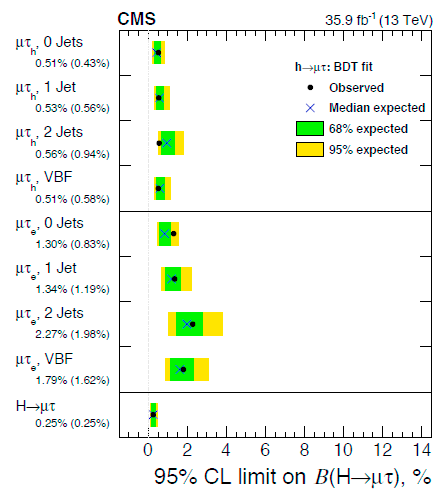
\includegraphics[width=0.4\textwidth]{plots/chapter2/BHmt.png}
  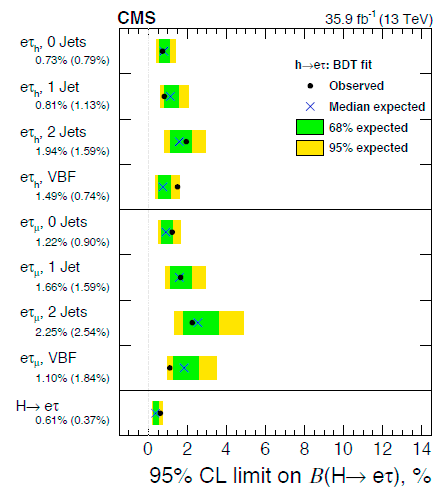
\includegraphics[width=0.4\textwidth]{plots/chapter2/BHet.png}
  \caption{Expected and observed 95\% CL upper limits by category of a search for LFV \Hmt and \Het decays with 2016 dataset \cite{Sirunyan:2019shc}.}
  \label{fig:bh}
\end{figure}
